\section{Methodology}
\label{sec:methodology}

In total, 360 runs were carried out in two measurement sessions.

\subsection{Setup}

The source of the handover is a browser application which boots a WebContainers instance and starts a heartbeat process inside it. Every \SI{100}{\milli\second}, the heartbeat ticks, which means it increments a counter and appends it as a timestamped line to a log file. Every \SI{1000}{\milli\second} the heartbeat writes the counter to a state file.

A local server acts as the runner (Figure~\ref{fig:setup}). It receives the exported archive and measures the duration of every phase. The runner reaches the target only through an adapter. This adapter is implemented for E2B as the measured target. 
The runner and a headless browser share one host in Northern Germany. One script controls the browser and runs the whole measurement session without manual intervention.

The target is a microVM of the default E2B template. It is created in us-west-1, the default region, as other regions have to be enabled by the support of E2B first \cite{e2b-client-2026,e2b-eu-region-2026,e2b-migrate-2026}. Therefore, every transfer travels from Northern Germany to the US west coast, and the network path is part of every measured time. The setup code and the measured data are available in a repository \cite{migration-without-memory-repo-github}.

\begin{figure}[t]
  \centering
  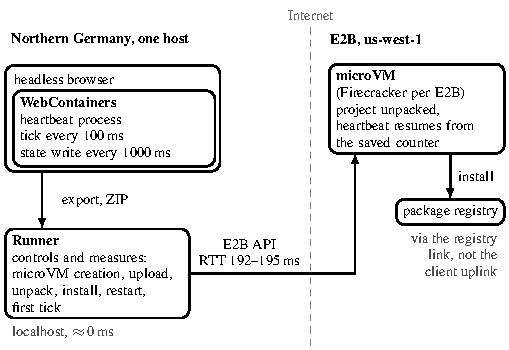
\includegraphics[width=\columnwidth]{figures/setup-diagram.pdf}
  \caption{Source, runner and target and their role in this setup.}
  \label{fig:setup}
\end{figure}

\subsection{Experimental design}

In the \textbf{size study}, two strategies are crossed with four project sizes, the size of the payload in the full copy. These four sizes are the levels small (\SI{1.8}{\kilo\byte}), light (\SI{0.91}{\mega\byte}), medium (\SI{4.62}{\mega\byte}) and large (\SI{13.93}{\mega\byte}). A cell is one strategy at one level. This gives eight cells at 30 repetitions and 240 runs. The script changes the order of the cells randomly within every cycle, in which each cell runs once. A handover can happen at any point between two state writes. Therefore, the script draws the stop offset, the time from the last state write to the stop, uniformly between 0 and \SI{1000}{\milli\second}. The order and the stop offsets come from a fixed seed, so the measurement session can be repeated.

\textbf{Manifest-based transfer} sends only the sources, the package manifest, the lockfile and the files of the heartbeat, \SIrange{1.7}{17.2}{\kilo\byte} in total.

The \textbf{live study}, named after live migration, is run on the large level only. The full copy transfers the most bytes at this level, so the push phase of pre-copy can move the most work before the stop. Two strategies with a push phase are added to the full copy and manifest-based transfer. At 30 repetitions each, this gives 120 runs, again with a fixed seed and a random order of the cells within every cycle. 
\textbf{Pre-copy} sends the full working directory to the target before the stop. 
\textbf{Manifest-push} sends it without the installed dependencies and runs the install on the target before the stop.

In every run, the browser page is reloaded, the WebContainers instance installs the dependencies of the level and the heartbeat starts. For the full copy and manifest-based transfer, the source stops the heartbeat at the drawn offset after three state writes. Afterwards, it exports the working directory and posts it to the runner. After the runner receives the archive, it creates a fresh microVM. Then it uploads and unpacks the archive and runs the install for manifest-based transfer. Lastly, it restarts the heartbeat from the exported state and waits for the first new tick. For pre-copy and manifest-push, the export, the microVM creation, the upload and the unpack take place before the stop. At the stop, only the files changed since the push follow, including the state file.

Each level carries at most one direct dependency with a fixed lockfile. The light level adds \texttt{express}, the medium level \texttt{@babel/preset-env} and the large level \texttt{aws-sdk}. These packages were chosen by their size and the duration of their install. The small level acts as a control without any dependency, so both strategies transfer about the same bytes. The light level installs 68 packages, the medium level 135 and the large level only 45.

\subsection{Dependent variables}

Four variables are recorded per run, and a fifth one for the strategies with a push phase. 
The \textbf{interruption time} runs from the stop on the source to the first tick on the target. It corresponds to the downtime in the migration literature \cite{clark2005live}. With a pull phase \cite{hines2009post}, it would only contain the files accessed before the first tick. After the restart, the heartbeat, whose first tick ends the interruption, accesses only three files. Hence, the interruption time of post-copy would hardly depend on the project size. Hybrid migration would fetch the files that pre-copy sends at the stop. Therefore, neither is measured, and the target needs no layer that fetches missing files on access.
With a push phase, the \textbf{total handover time} adds the push phase to the interruption time. Without a push phase, it equals the interruption time. It is split into the phases transfer, install, target start and harness. The target start consists of microVM creation, restart of the heartbeat and first tick. The transfer consists of export, upload and unpack. The harness is the overhead of the measurement setup.

The \textbf{bytes transferred} are the size of the archive which crosses the boundary. For the strategies with a push phase, this is the archive sent at the stop. The \textbf{state loss} is the number of ticks between the last state write and the stop, both read on the source after the stop. 
Lastly, the \textbf{source shortfall} compares the ticks of the source during the push phase with the ticks expected at its idle rate. The idle rate is the number of ticks per second the heartbeat reaches when the source does nothing else. It is measured as the increase of the state loss per second of stop offset over the 120 runs of the live study.

Each run is correct if the target loads the exported counter and keeps counting.

\subsection{Interruption time across two clocks}

The interruption time starts with a timestamp right before the stop on the source and ends with the first new line in the log of the heartbeat on the target. In all 360 runs, the clocks of the browser and the runner differ by $-0.5$ to \SI{+0.5}{\milli\second}, which is the resolution of the measurement. Therefore, only the clock of the target is converted to the clock of the runner. Its offset is estimated in every run with Cristian's method. The runner asks the target for its time and measures the round trip of this request. The target reads its clock at some point within this round trip, so the estimate is off by at most half of it \cite{cristian1989probabilistic}. The runner reads the clock five times and keeps the reading with the shortest round trip, without considering clock drift.

\subsection{Statistical treatment}
The interruption time and the state loss are reported as medians, the phases of the total handover time in Figure~\ref{fig:decomposition} as means. The dispatch of the restart command, from its call at the runner to its start on the target, is bimodal in all twelve cells. Therefore, medians, a bootstrap confidence interval and a permutation test are used, as none of them assumes a normal distribution. According to Papadopoulos et al., such data may need methods without this assumption, and bootstrap sampling can make the evaluation more robust \cite{papadopoulos2019methodological}.

RQ-2 is answered by a bootstrap confidence interval and a two-sided permutation test on the median difference between the strategies per level. Both use 10,000 draws and a fixed seed. The interval is the 2.5th to 97.5th percentile of the bootstrap distribution, and no correction is applied across the four levels. The crossing point is placed on a straight line between the two adjacent levels at which the median difference changes sign. Its interval comes from the same bootstrap draws. In both measurement sessions, the full copy and manifest-based transfer run at the large level. The intervals of their differences are too wide to show that the measurement sessions are the same. Therefore, cells are compared only within a study.

In the live study, the primary comparisons were fixed before the measurement session. These are pre-copy against the full copy and manifest-push against manifest-based transfer on the interruption time. They use the same bootstrap interval and permutation test. The comparison of pre-copy with manifest-push and every comparison of the total handover time are post hoc. Furthermore, no run is discarded.
